% Marius-Juston 2026
\documentclass[border=10pt]{standalone}
\usepackage{tikz}

\begin{document}

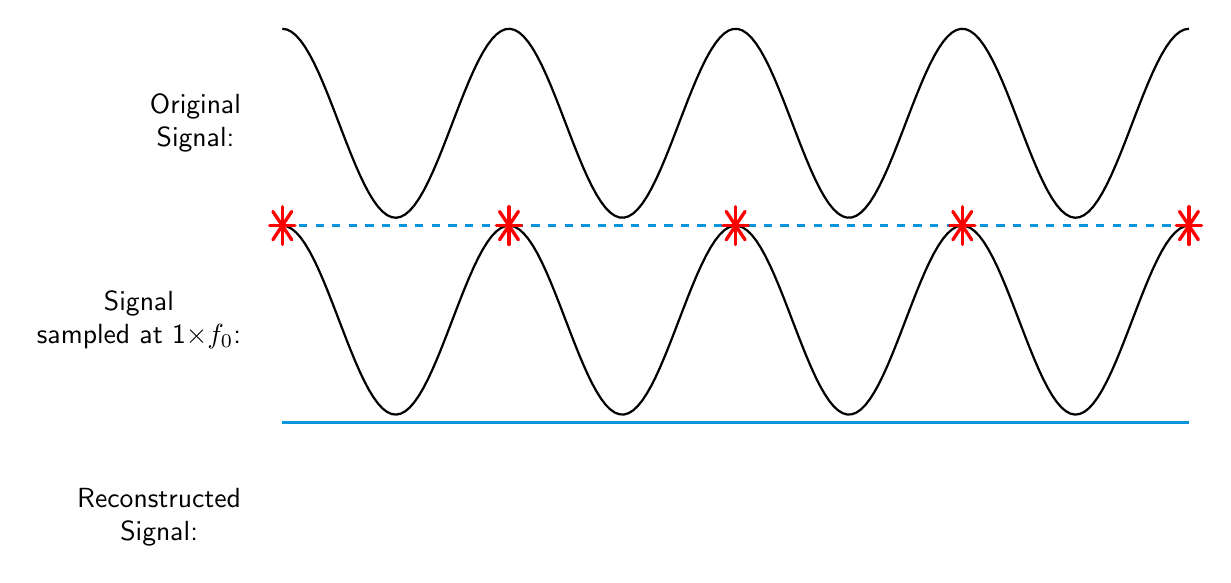
\begin{tikzpicture}[x=0.8cm, y=1.2cm]
  \sffamily
  
  % =======================================================
  % PARAMETERS
  % =======================================================
  % Define the sampling frequency ratio (e.g., 2.0 = Nyquist critical limit)
  \def\FsRatio{1} 
  
  % Define the phase offset in degrees (90 degrees = 0.25 of a period)
  \def\PhaseOffset{90}
  
  \def\Nperiods{4} % Number of fundamental waveform periods to display
  \def\Xmax{\Nperiods * 360}
  \def\Xscale{0.01} % Scaling factor for mapping degrees to cm
  
  % Dynamically calculate degree steps per sample and total valid samples
  \pgfmathsetmacro{\StepDeg}{360 / \FsRatio}
  \pgfmathtruncatemacro{\TotalSamples}{floor(\Nperiods * \FsRatio)}

  % Calculate initial Y-value based on phase offset
  \pgfmathsetmacro{\Yinit}{sin(\PhaseOffset)}

  % =======================================================
  % 1. Original Signal
  % =======================================================
  \begin{scope}[yshift=5cm]
      \node[align=center, left] at (-0.5, 0) {Original\\Signal:};
      \draw[thick] plot[domain=0:\Xmax, samples=200] ({\x*\Xscale}, {sin(\x + \PhaseOffset)});
  \end{scope}

  % =======================================================
  % 2. Sampled Signal (at \FsRatio * f0)
  % =======================================================
  \begin{scope}[yshift=2.5cm]
      \node[align=center, left] at (-0.5, 0) {Signal\\sampled at \FsRatio$\times f_0$:};
      
      % Underlying continuous signal
      \draw[thick] plot[domain=0:\Xmax, samples=200] ({\x*\Xscale}, {sin(\x + \PhaseOffset)});
      
      % First-Order Hold (FOH) Dashed interpolation path
      \draw[cyan!80!blue, very thick, dashed] (0, \Yinit)
      \ifnum\TotalSamples>0
          \foreach \k in {1,...,\TotalSamples} {
              -- ({\k * \StepDeg * \Xscale}, {sin(\k * \StepDeg + \PhaseOffset)})
          }
      \fi;
      
      % Convolution Dirac markers (Red 8-point asterisks)
      \foreach \k in {0,...,\TotalSamples} {
          \pgfmathsetmacro{\xval}{\k * \StepDeg}
          \pgfmathsetmacro{\yval}{sin(\xval + \PhaseOffset)}
          \begin{scope}[shift={({\xval*\Xscale}, \yval)}]
              \draw[red, very thick, line cap=round] (-0.15, -0.15) -- (0.15, 0.15);
              \draw[red, very thick, line cap=round] (-0.15, 0.15) -- (0.15, -0.15);
              \draw[red, very thick, line cap=round] (0, -0.2) -- (0, 0.2);
              \draw[red, very thick, line cap=round] (-0.2, 0) -- (0.2, 0);
          \end{scope}
      }
  \end{scope}

  % =======================================================
  % 3. Reconstructed Signal (FOH Output)
  % =======================================================
  \begin{scope}[yshift=0cm]
      \node[align=center, left] at (-0.5, 0) {Reconstructed\\Signal:};
      
      % Continuous linear interpolation output
      \draw[cyan!80!blue, very thick] (0, \Yinit)
      \ifnum\TotalSamples>0
          \foreach \k in {1,...,\TotalSamples} {
              -- ({\k * \StepDeg * \Xscale}, {sin(\k * \StepDeg + \PhaseOffset)})
          }
      \fi;
  \end{scope}

\end{tikzpicture}

\end{document}